% chapter3.tex
% Capitulo 3. Estudio de la plataforma USRP y GNURadio
%==========================================================================
\chapter{Estudio de la plataforma USRP y GNURadio}

En este cap\'itulo se aplican los conceptos de la modulaci\'on QPSK para
analizar el rendimiento de la plataforma USRP. El experimento consta de elaborar
un programa que realice la modulaci\'on utilizando el lenguaje Python y
\gnuradio\ bajo el ambiente Linux. Este programa va interactuar con el USRP
por medio del puerto USB, intercambiando la informaci\'on que se transmite y
recibe. El an\'alisis ser\'a visualizado en la PC utilizando las herramientas
que \gnuradio\ proporciona.

La transmisi\'on se realizar\'a utilizando las tarjetas LFTX y LFRX. Estas
tarjetas proporcionan acceso directo a las salidas del DAC y entradas del ADC
respectivamente sin ning\'un tipo de amplificaci\'on y filtrado. Dependiendo la
aplicaci\'on ser\'a necesario acoplar una etapa de RF para acondicionar la
se\~nal y poder ser transmitida correctamente.

% 3.1. Estructura del sistema USRP
%==========================================================================
\section{Estructura del sistema USRP}

El sistema USRP es un dispositivo que permite dise\~nar radios reconfigurables
por software. El dispositivo es solamente una parte de la estructura completa de
un SDR. Su funci\'on principal es actuar como la secci\'on de frecuencia intermedia de un sistema de
comunicaciones.

La figura \ref{fig:sisusrp} muestra los componentes que forman un sistema de
comunicaciones implementado con el USRP. Todo el procesamiento en banda base, es decir,
modulaciones, codificaciones, etc., es llevado a cabo en una PC x86. Esta PC
contiene el programa Python que realiza todo el procesamiento digital con la
se\~nal o se\~nales que se desean trabajar. Esto se lleva a cabo utilizando las
herramientas proporcionadas por \gnuradio.

\begin{figure}[t]
\centering
	\includegraphics[width=5.5in]{figs/usrp}
	\caption{Placa principal del USRP.}
	\label{fig:sisusrp}
\end{figure}

Los componentes principales del USRP son el FPGA Altera Cyclone EP1C12, los codec AD9862 de alta
velocidad , las interfaces de las tarjetas auxiliares y el controlador Cypress FX2 para la
comunicaci\'on por el puerto USB. La tarjeta cuenta con 4 conectores donde se pueden conectar 2
tarjetas TX y 2 RX o 2 tarjetas RFX (transmisor y receptor en una sola tarjeta auxiliar). Cada
tarjeta puede acceder a dos de los 4 ADC/DACs. Si la tarjeta utiliza muestreo real (sin usar IQ)
entonces esto permitir\'a tener 2 secciones de RF independientes, para un total de 4. Si se utiliza
muestreo complejo IQ entonces cada tarjeta tendra una sola etapa de RF, para un total de 2 en todo
el sistema. Cada tarjeta auxiliar tiene dos conectores SMA para transmitir o recibir se\~nales y una
EEPROM con bus de datos I2C que identifica la tarjeta al sistema. Esto permite que el software en la
PC pueda configurar el sistema basandose en la tarjeta que este instalada. Las tarjetas que
actualmente soporta el USRP se muestran en la tabla \ref{tbl:cards}.

\begin{table}[htp]
\begin{center}
	\begin{tabular}{|c|p{8cm}|p{3cm}|}
		\hline
		\textbf{Tarjeta} & \textbf{Descripci\'on} & \textbf{Frecuencia de operaci\'on}\\
		\hline
		BasicTX y RX & Transmisor y Receptor para ser utilizados con equipo externo de RF. Sus salidas
		estan acopladas por un transformador directamente a los ADC/DACs con una impedancia de 50$\Omega$.
		& 1Mhz-250Mhz\\
		\hline
		LFTX y LFRX & Similar al BasicTX y RX pero las salidas estan acopladas por amplificadores
		diferenciales en lugar de transformadores. Esto las permite trabajar con frecuencias hasta DC.
		Tambien cuentan con un filtro pasabajas con frecuencia de corte de 30Mhz. & DC-30Mhz\\
		\hline
		TVRX & Sistema receptor de VHF y UHF basando en un sintonizador de TV con un ancho de banda de
		canal de 6Mhz. & 50Mhz-860Mhz\\
		\hline
		DBSRX & Sistema receptor con filtro de canal controlado por software de 1Mhz a 60Mhz. &
		800Mhz-2.4Ghz\\
		\hline
		RFX400 & TX y RX en una sola tarjeta con un ancho de banda de canal de 30Mhz. & 400Mhz-500Mhz\\
		\hline
		RFX900 & TX y RX con 200mW(23dBm) de potencia.  & 750Mhz-1050Mhz\\
		\hline
		RFX1200 & TX y RX con 200mW de potencia que cubre las bandas satelitales. & 1150Mhz-1450Mhz\\
		\hline
		RFX1800 & TX y RX con 100mW(20dBm) de potencia & 1.5Ghz-2.1Ghz\\
		\hline
		RFX2400 & TX y RX con 50mW(17dBm) de potencia con un filtro pasa bandas alrededor de la banda
		ISM(2400-2433Mhz). El filtro se puede desabilitar para utilizar todo el rango de frecuencias. &
		2.3Ghz-2.9Ghz\\
		\hline
		XCVR2450 & TX y RX que cubre toda la banda ISM asi como tambien algunas bandas japonesas. &
		2.4-2.5Ghz y 4.9-5.9Ghz\\
		\hline
		WBX & TX y RX que cubre varias bandas incluyendo televisi\'on, comunicaciones m\'obiles, sensores
		inal\'ambricos, etc. & 50Mhz-2.2Ghz\\
		\hline
	\end{tabular}
	\vspace{0.5in}
	\caption{Tarjetas auxiliares que soporta el USRP.}
	\label{tbl:cards}
\end{center}
\end{table}

El controlador FX2 integra un CPU 8051 con un controlador de USB de alta velocidad que implementa 3
\emph{endpoints} logicos para la comunicaci\'on con el FPGA y la PC como se describen en la tabla
\ref{tbl:endpoints}.Cada \emph{endpoint} establece una via de comunicaci\'on entre el dispostivo
USB y el \emph{host}. El endpoint 0 es el de control y es necesaria su implementaci\'on para que el
dispositivo pueda ser compatible y a su vez, ser certificado por el est\'andar de USB \cite{usb}.
Los endpoints 2 y 6 son de tipo Bulk, que de acuerdo a la especificaci\'on del USB, son los que
permiten el mayor rendimiento de transferencia (512 bytes por paquete). Estos son utilizados para
enviar los datos de la se\~nal al FPGA. El FX2 utiliza una interfaz de prop\'osito gen\'erico (GPIF)
para proporcionar un bus de datos al mundo exterior, esto con el prop\'osito de facilitar la
interfaz a otros dispositivos. En este caso el GPIF se conecta directamente al FPGA con una tasa de
transferencia de 96 MB/sec.

\begin{table}[htp]
\begin{center}
	\begin{tabular}{|c|c|}
		\hline
		\textbf{Endpoints} & \textbf{Descripci\'on} \\
		\hline
		0 & Control/Status \\
		\hline
		2 & PC $\rightarrow$ FPGA \\
		\hline
		6 & FPGA $\rightarrow$ PC \\
		\hline
	\end{tabular}
	\vspace{0.5in}
	\caption{\emph{Endpoints} implementados por el controlador FX2}
	\label{tbl:endpoints}
\end{center}
\end{table}

El FPGA es el encargado de realizar operaciones de alta velocidad y de reducir
la tasa de datos en una m\'as adecuada para que la se\~nal pueda ser transferida
por el puerto USB. Para la etapa de RX, la configuraci\'on b\'asica contiene dos
convertidores digirales hacia abajo (DDC) implementados con filtros CIC (Peine
Integradores en Cascada) de 4 etapas y filtros de media banda (\emph{Half-band}
o HB) de orden 31. El prop\'osito del DDC es transformar la se\~nal pasa bandas a banda base. Esto
se logra centrando su frencuencia en 0Hz, as\'i eliminando la portadora. La estructura del
DDC se muestra en la figura \ref{fig:ddcblock}.

\begin{figure}[htp]
\centering
	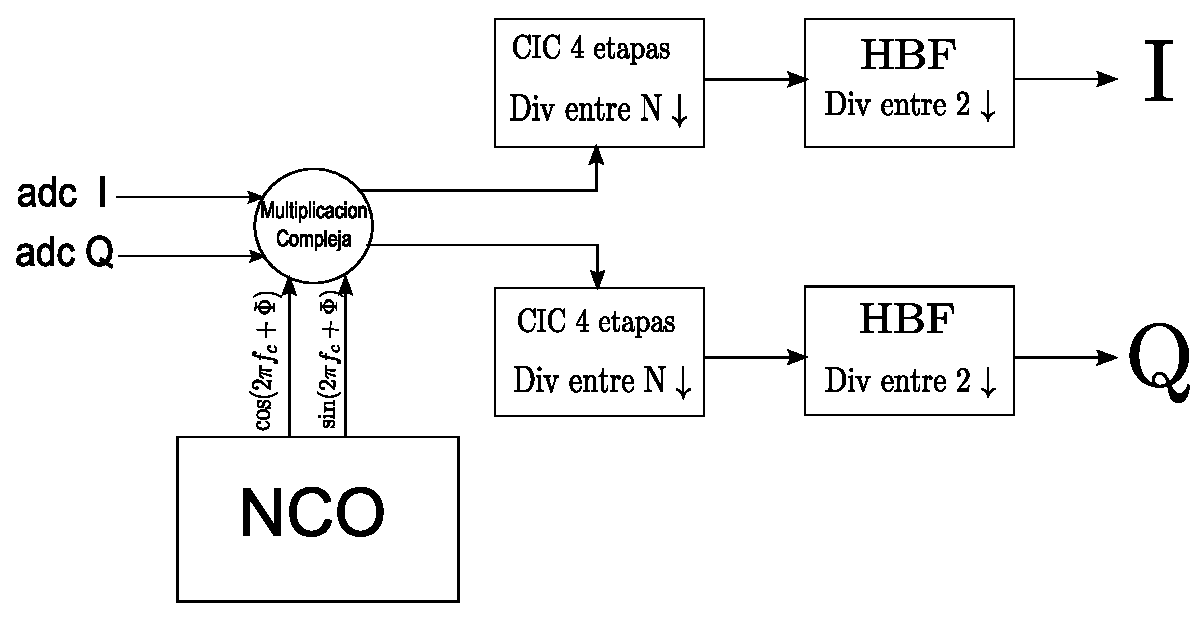
\includegraphics[width=5.5in]{figs/ddc}
	\vspace{0.3in}
	\caption{Estructura del DDC implementado en el USRP}
	\label{fig:ddcblock}
\end{figure}

EL USRP, en su configuraci\'on b\'asica, usa dos DDCs, cada uno con 2
entradas. La se\~nal compleja que entregan los ADCs es multiplicada por otra se\~nal con una
frecuencia intermedia constante generada por un oscilador controlado numericamente (NCO).  La
se\~nal resultante se encuentra ahora centrada en 0Hz. Despu\'es es introducida al filtro CIC para
realizar una decimaci\'on por $N$, donde $N$ es especificado por el usuario desde el programa
del usuario. La funci\'on de transferencia del filtro CIC es la siguiente
\cite{cic}:

\begin{equation}
H(z)=H_I^N(z)H_C^N(z)=\frac{(1-z^{-RM})^N}{(1-z^{-1})^N}=\left(\sum_{k=0}^{RM-1}z^{-1}\right)^N
\end{equation}

\begin{equation*}
\begin{aligned}
\text{Donde: }H_I^N&=\text{es la funci\'on de transferencia de la etapa
integradora}\\
H_C^N&=\text{es la funci\'on de transferencia de la etapa filtro comb}\\
R&=\text{es la tasa de decimaci\'on o interpolaci\'on}\\
M&=\text{n\'umero de muestras por etapa}\\
N&=\text{n\'umero de etapas por filtro}
\end{aligned}
\end{equation*}

El USRP implementa este filtro con los siguientes par\'ametros: $R$ = variable (4 m\'inimo), $M$ = 1
y $N$ = 4. La respuesta a la frecuencia de esta configuraci\'on se muestra en la
\ref{fig:cicresp}.

\begin{figure}[hpt]
\centering
	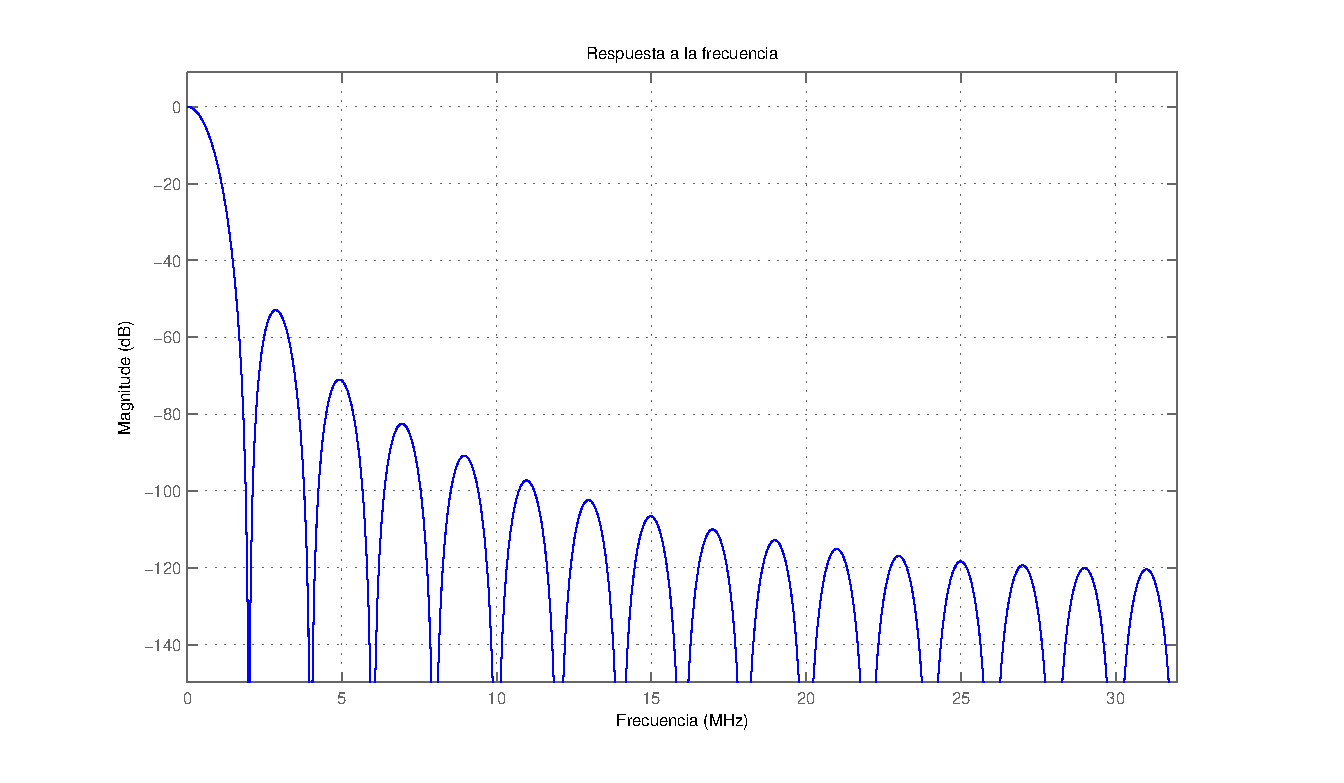
\includegraphics[width=5.9in]{figs/cicresponse}
	\caption{Respuesta a la frecuencia del filtro CIC de 4 etapas y R =	4}
	\label{fig:cicresp}
\end{figure}

La \'ultima etapa del DDC es el filtro HB el cual realiza una decimaci\'on de 2
y ayuda a rechazar cualquier banda no deseada por las operaciones previas. La
funci\'on de transferencia del filtro HB \cite{nguyen} es la
siguiente:

\begin{equation}
H(z)=\sum_{n=0}^{N-1}h(n)z^{-n}
\end{equation}

Estos filtros tienen las siguientes restricciones:

\begin{itemize}
  \item N-1 debe ser par
  \item $h(n)=h(N-1-n)$
\end{itemize}

La respuesta a la frecuencia es

\begin{equation}
H(e^{j\omega})=e^{-j\omega N-1/2}H_0(e^{-j\omega})
\end{equation}

donde $H_0(e^{-j\omega})$ representa la respuesta a la amplitud con valor real.

\begin{figure}[hpt]
\centering
	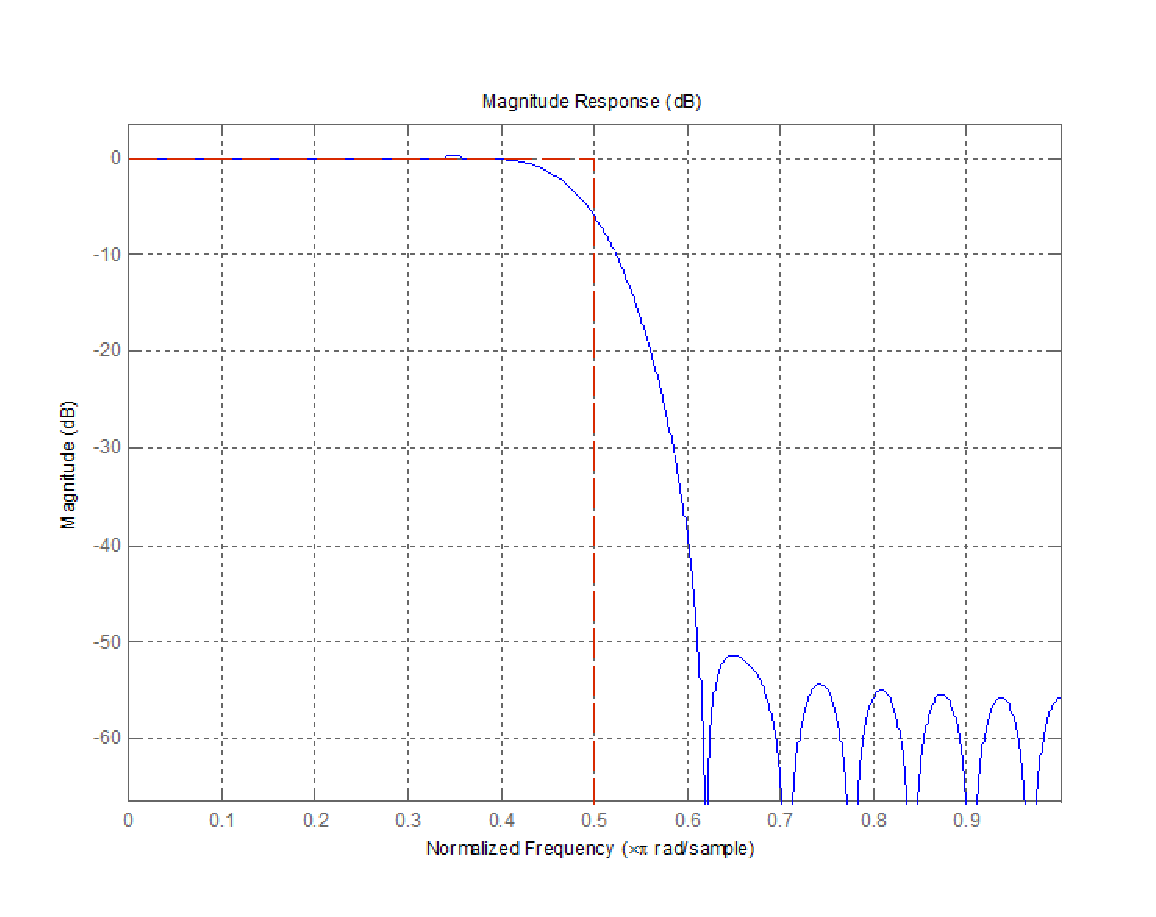
\includegraphics[width=5.9in]{figs/hbresponse}
	\caption{Respuesta a la frecuencia del filtro de media banda}
	\label{fig:hbresp}
\end{figure}

Las caracter\'isticas del filtro HB de acuerdo al USRP son las siguientes:

\begin{itemize}
  \item Orden 31
  \item Decimador 2
  \item Pasa bajas
\end{itemize}

En la figura \ref{fig:hbresp} se muestra la respuesta a la frecuencia del filtro HB.
Existe simetr\'ia con respecto a la banda $\pi /2$. Esta es una de las
caracter\'isticas de estos filtros. Debido a esa simetr\'ia la respuesta al
impulso es

\begin{equation}
h(n)=\left\{
\begin{array}{l l}
0, & \quad n=\frac{N-1}{2}=\text{par y diferente a 0}\\
\frac{1}{2}, & \quad n=\frac{N-1}{2}
\end{array}\right.
\end{equation}

Debido a esta simetr\'ia estos filtros son muy eficientes y f\'aciles de
implementar ya que aproximadamente el 50\% de sus coeficientes son 0.

La combinaci\'on del filtro CIC y HB dan un factor de decimaci\'on m\'inimo de
8. El ADC tiene una taza de muestreo de 64Ms/S, por lo tanto, el ancho de banda
total ser\'a de 32Mhz. Los datos enviados son de 16 bits para I y Q, \'osea, 4
bytes por muestra compleja. Esto resulta en un ancho de banda efectivo de 8Mhz
(32Mhz/4bytes). El rango de decimaci\'on que soporta el USRP es [8, 256].

Para la etapa de TX el proceso es el inverso. El FPGA contiene filtros CIC interpoladores que se
encargan de interpolar la se\~nal, elevarla a la frecuencia intermedia y despu\'es
enviarla a los DACs. El proceso de conversi\'on digital hacia arriba (DUC)
est\'a contenido en el chip AD9862 y no en el FPGA como lo es en el proceso de
RX. Este chip contiene ambos ADCs y DACs pero \'unicamente en la etapa del TX
realiza alg\'un otro procesamiento sobre la se\~nal. La frecuencia de muestreo
de los DACs es de 128MS/s de 14 bits cada uno, d\'andonos una frecuencia Nyquist
de 64MS/s. La salida proporciona 1V pico a una carga diferencial de 50$\Omega$.
Existe un amplificador de ganancia programable (PGA) que puede proporcionar
hasta 20dB de ganancia y es programable por software. Las se\~nales del DAC son
en base a corriente y varean entre 0 y 20mA.

% \begin{figure}[hpt]
% \centering
% 	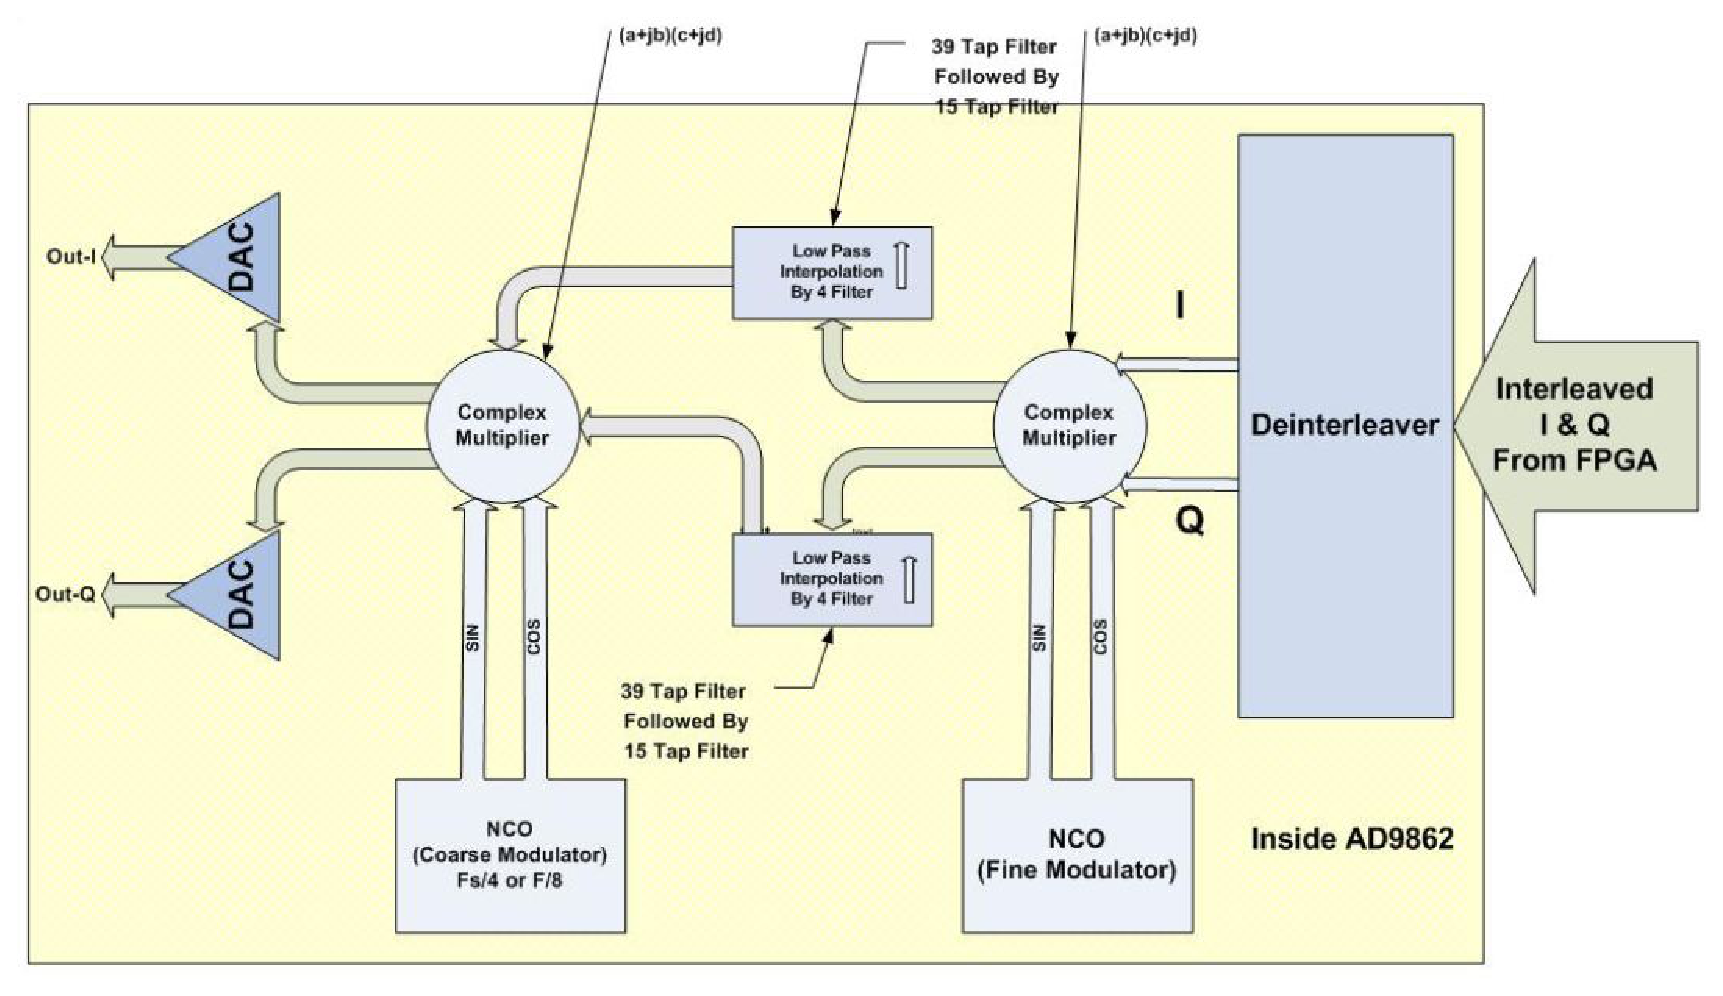
\includegraphics[width=5.5in]{figs/duc}
% 	\vspace{0.2in}
% 	\caption{Estructura del DUC implementado en el AD9862}
% 	\label{fig:ducblock}
% \end{figure}

% 3.2. GNURadio
%==========================================================================
\section{GNURadio}
\label{sec:gnuradio}

El USRP fue dise\~nado para ser utilizado principalmente, pero no
exclusivamente, por la herramienta de desarrollo \gnuradio. Esta
herramienta es abierta (\emph{Open Source}) y consiste en un sistema de
procesamiento de se\~nales implementado a base de bloques que se ligan uno con
el otro para formar un sistema completo de comunicaciones. Las aplicaciones que
se desarrollan son principalmente implementadas con el lenguaje Python, mientras
que las operaciones cr\'iticas de procesamiento de se\~nales son implementadas
en C++ utilizando las extensiones de punto flotante del CPU si es que est\'an
presentes. Cabe mencionar que aunque la funci\'on principal de esta herramienta
no es realizar simulaciones, tiene la capacidad de generar sistemas de
comunicaciones utilizando datos obtenidos previamente por medio de alguna
simulaci\'on o generador. Esto es \'util cuando no se cuenta con hardware de RF
para llevar a cabo la aplicaci\'on.

\gnuradio\ no est\'a limitado a trabajar \'unicamente con el USRP. Debido a
la naturaleza abierta de la herramienta, uno puede dise\~nar su propio bloque
que encapsule alg\'un hardware especial. La programaci\'on del driver se lleva a
cabo en C, es encapsulada con las clases de C++ para implementar el bloque y
despu\'es es encapsulada nuevamente en Python para ser utilizado en la
aplicaci\'on general. De esta manera el usuario no se preocupa por los detalles
del funcionamiento del hardware, \'unicamente le proporciona los par\'ametros
adecuados al bloque y este se encarga de establecer la comunicaci\'on adecuada.

% Programacion en GNURadio con Python
%==========================================================================
\section{Programaci\'on en GNURadio con Python}

Como se menciono en el captulo \ref{sec:gnuradio}, la programaci\'on se lleva a
cabo principalmente en el lenguaje Python. El lenguaje C++ tambi\'en se utiliza
pero \'unicamente si se desea desarrollar un modulo nuevo o modificar algunos de
los que ya existen.

\gnuradio es un conjunto de m\'odulos de Python con la capacidad de
realizar diversas operaciones de procesamiento digital de se\~nales para el desarrollo de
sistemas de radios configurables por software. Es posible mesclar diferentes
m\'odulos de otros \emph{frameworks} o librer\'ias junto con los de \gnuradio\
para incluir mayor soporte al que se ofrece.

El concepto que se aplica para los programas realizados con esta librer\'ia es
el de grafos. Cada aplicaci\'on cuenta con una serie de nodos o bloques
conectados entre s\'i para crear una cadena completa de RF llamado grafo de
flujo. Los bloques se encargan de realizar alguna operaci\'on sobre la
informaci\'on que fluye atreves de la grafica y est\'os pueden ser operaciones
matem\'aticas, envi\'o de datos a alg\'un puerto, etc., mientras que las aristas
transportan la informaci\'on entre los nodos. Cada bloque tiene definido una
serie de puertos de entradas y salidas las cuales aceptan y entregan un tipo de
datos espec\'ifico. No es posible realizar una conexi\'on entre dos puertos con
tipos de datos incompatibles. Un ejemplo de una grafica de flujo sencilla se
muestra en la figura \ref{fig:radioflow}.

\begin{figure}[hpt]
  \centering
  \vspace{0.3in}
	\begin{tikzpicture}
		\node (sg) [grblock] {\small{Generador de se\~nales}};
		\node (os) [grblock, right=of sg] {\small{Osciloscopio}}
		edge [<-] (sg);
		\node (fft) [grblock, below=of os] {FFT};
		\draw[->] (sg) |- (fft);
		\node (os2) [grblock, right =of fft] {\small{Osciloscopio}}
		edge [<-] (fft);
	\end{tikzpicture}
	\vspace{0.5in}
	\caption{Ejemplo de una grafica de flujo en \emph{GNURadio}}
	\label{fig:radioflow}
\end{figure}

La informaci\'on que viaja a trav\'es de las aristas puede provenir de una fuente
externa \'o interna. Para el caso de las fuentes internas estas generan se\~nales
puramente digitales a trav\'es de m\'etodos de procesamiento digital de
se\~nales. Las fuentes externas primeramente adquieren una se\~nal an\'aloga por
medio de alguna interfaz delantera. Esta interfaz se encarga del
acondicionamiento de la se\~nal y de su digitalizaci\'on por medio de un ADC
para luego ser procesada por el bloque de \gnuradio. Estos conceptos se
aplican igualmente para bloques de salidas. Estos bloques pueden llevar sus
datos a alg\'un archivo, desplegarlos en forma de alguna grafica o sacarlos a
trav\'es de alguna interfaz por medio de un DAC y luego al mundo exterior. Un
ejemplo de un programa que ilustra estos conceptos se muestra en el listado
\ref{ex:radioexp}. Este programa utiliza dos bloques que generan dos se\~nales
senoidales independientes a diferentes frecuencias y las entrega a un bloque de audio que
representa la tarjeta de sonido de la PC donde se est\'a ejecutando el programa,
esto en efecto mezcla ambas se\~nales para producir un tono.

\begin{lstlisting}[float,frame=single,label=ex:radioexp,caption={Ejemplo de programa utilizando \gnuradio}] 
from gnuradio import gr 
from gnuradio import audio

class my_top_block(gr.top_block):
    def __init__(self):
      gr.top_block.__init__(self)

      sample_rate = 32000
      ampl = 0.1

      src0 = gr.sig_source_f (sample_rate, gr.GR_SIN_WAVE, 350, ampl)
      src1 = gr.sig_source_f (sample_rate, gr.GR_SIN_WAVE, 440, ampl)
      dst = audio.sink (sample_rate, "")
      self.connect (src0, (dst, 0))
      self.connect (src1, (dst, 1))

if __name__ == '__main__':
     try:
       my_top_block().run()
     except KeyboardInterrupt:
       pass
\end{lstlisting}

El programa se inicia importando los m\'odulos necesarios para la aplicaci\'on.
Aqu\'i se importa el modulo \verb|gnuradio| y dos de sus submodulos: \verb|gr| y
\verb|audio|. Despu\'es se declara una clase que se deriva de \verb|top_block|.
Todas las clases de \gnuradio\ se tienen que derivar de
\verb|top_block| o de \verb|hier_block2| ya que estas dos clases act\'uan como
un contenedor para la grafica de flujo. La primera clase act\'ua como un
contenedor para una \'unica grafica y la segunda soporta el desarrollo de
graficas jer\'arquicas.

Los bloques y sus conexiones se definen dentro del constructor de la clase, en
este caso es la funci\'on \verb|__init__|. Esta l\'inea de c\'odigo tambi\'en
manda llamar la funci\'on \verb|__init__| de la clase de la que se deriva,
pas\'andole los par\'ametros que sean necesarios (si es que los pide). Esto es
necesario para llevar a cabo la inicializaci\'on de ambas clases. En las
siguientes dos l\'ineas se declaran dos variables para llevar el control del
tiempo de muestro y de la amplitud. Las siguientes dos l\'ineas demuestran la
manera de c\'omo se declaran los bloques de ejecuci\'on. Cada bloque est\'a
representado por una clase y su inicializaci\'on consta en mandar llamar su
constructor con los par\'ametros necesarios para su funcionamiento. Como se
puede observar, ambos bloques se encuentran dentro del submodulo \verb|gr| y su
constructor se invoca con los par\'ametros que requieren para generar el tipo de
se\~nal que deseamos. Para estos bloques los par\'ametros son los siguientes en
orden: el tiempo de muestreo, una constante que indica el tipo de se\~nal que se
desea generar (estas constantes tambi\'en se encuentran dentro del submodulo
\verb|gr|), la frecuencia de la se\~nal y su amplitud. La siguiente l\'inea
declara un tercer bloque que es el de audio y representa la tarjeta de sonido de
la PC. Los par\'ametros que necesita son el tiempo de muestreo y el nombre del
dispositivo de audio (esto es en caso de que se tenga m\'as de uno en la PC).

Por \'ultimo las dos siguientes l\'ineas demuestran la manera de c\'omo hacer
las conexiones entre los bloques. Como la clase fue derivada de \verb|top_block|
ahora contamos sus funciones para nuestro uso. Una de estas funciones se llama
\verb|connect| y se utiliza para conectar cada uno de los bloques. Los
par\'ametros que acepta son clases derivadas de los bloques principales o tuplas
con dos elementos, el bloque y un entero. El entero se utiliza para indicar que
puerto utilizar para la conexi\'on donde esto es \'unicamente valido para
bloques que acepten m\'as de una conexi\'on a la vez.  La numeraci\'on de los
puertos inicia con cero por lo que la primera conexi\'on lleva la primera
se\~nal al puerto 0 y la segunda conexi\'on lleva la segunda se\~nal al puerto
1.

\begin{figure}[hptb]
\vspace{0.3in}
\centering
	\begin{tikzpicture}[node distance=15mm and 20mm]
	\node (sg) [grblock] {\footnotesize{Gr.signal\_source\_f\\
						Amp=1\\
						Freq=350Hz}};
	\node (sg2) [grblock, below=of sg] {\footnotesize{Gr.signal\_source\_f\\
						Amp=1\\
						Freq=440Hz}};
	\node (as) [grblock, below right=of sg, yshift=1.7cm] {\small{Audio.sink}};
	\draw [->] (sg.east) -- ++(1,0) |- (as);
	\draw [->] (sg2.east) -- ++(1,0) |- (as);
	\end{tikzpicture}
\vspace{0.5in}
\caption{Grafica de flujo del programa ejemplo.}
\label{fig:gnuradioexam}
\end{figure}

Despu\'es de la declaraci\'on de nuestro bloque principal, el programa se
ejecuta declarando una instancia de nuestra clase, y mandando llamar su
funci\'on run. Esta funci\'on tambi\'en es proporcionada por la clase
\verb|top_block|. Cuando este programa se ejecute el resultado debe ser un tono
emitido a trav\'es de las bocinas de la PC a la frecuencia de las dos se\~nales
generadas. La grafica representativa de este programa se muestra en la figura
\ref{fig:gnuradioexam}.

% Descripcion del experimento
%==========================================================================
\section{Descripci\'on del hardware y software}
En esta secci\'on se describe la manera en como se llev\'o a cabo el experimento para la
implementaci\'on de una transmisi\'on digital utilizando el esquema de modulaci\'on QPSK. Las
instrucciones para instalar el ambiente de desarrollo se describen a detalle en el apendice
\ref{AppA}.

\subsection{Hardware utilizado}
Los componentes que forman la parte de hardware son los siguientes:

\begin{itemize}
  \item USRP
  \item Tarjetas auxiliares LFTX y LFRX
  \item Cable coaxial SMA-SMA
  \item Cable USB
  \item Fuente de alimentaci\'on
\end{itemize} 

Como se describi\'o en la tabla \ref{tbl:cards}, las tarjetas LFTX y LFRX tienen un ancho de banda
de DC-30Mhz. Las terminales de estas tarjetas son de tipo SMA con una impedancia de 50$\Omega$. El
cable coaxial se utiliz\'o para minimizar perdidas en la transmisi\'on durante la caracterizaci\'on
del sistema. El cable USB es un cable tipo A-B (conectar estandar A a B). Las especificaciones de la
fuente de alimentaci\'on para el USRP son 6V @ 4A AC/DC. El sistema es capaz de operar en el rango
de 90-260VAC @ 50/60Hz lo cual permite que funcione en diferentes paises.

%TODO: Agregar imagen de las conecciones internas del usrp aqui. Tambien anexar expliacion.

\subsection{Codigo fuente de GNURadio}
El c\'odigo fuente de \gnuradio proporciona varios ejemplos que implementan varios conceptos
utiliznado los bloques de procesamiento que proporciona el \emph{framework}. Algunos de estos
ejemplos son: receptor de FM, decodificador de se\~nales ATSC, captura y analisis de audio,
modulacion OFDM, etc. La compilaci\'on del codigo fuente genera tambien la documentaci\'on de todos
los bloques de procesamiento, el cual es muy \'util como referencia mientras se desarrolla cualquier
aplicaci\'on. La estructura de los directorios que contienen los ejemplos se muestra en la figura
\ref{fig:extree}.

\begin{figure}[ht]
%\DTsetlength{0.2em}{1em}{0.2em}{0.4pt}{1.6pt} Valores default
\DTsetlength{1.5em}{1em}{0.2em}{0.4pt}{1.6pt} %offset, width, sep, rule-width, dot-size
	\dirtree{%
	.1 gnuradio-examples.
	.2 c++.
	.3 dial\_tone.
	.2 grc.
	.3 audio.
	.3 demod.
	.3 simple.
	.3 trellis.
	.3 usrp.
	.3 xmlrpc.
	.2 python.
	.3 apps.
	.4 hf\_explorer.
	.4 hf\_radio.
	.3 audio.
	.3 digital.
	.3 digital-bert.
	.3 mp-sched.
	.4 perf-data.
	.3 multi-antenna.
	.3 multi-usrp.
	.3 network.
	.3 ofdm.
	.3 pfb.
	.3 usrp.
	.3 usrp2.
	}
	\vspace{0.5in}
	\caption{\'Arbol de directorios de los ejemplos que ofrece \emph{GNURadio}}
	\label{fig:extree}
\end{figure}

El experimento se bas\'o en el ejemplo del directorio \verb|digital|. Este programa implementa un
transmisor completo utilizando varias modulaciones digitales como GMSK, BPSK y QPSK y viene en dos
versiones: una se maneja a trav\'es de una consola de comandos y la otra implementa una interfaz de
usuario utiliando la libreria QT que ayuda a visualizar de manera grafica lo que el sistema esta
recibiendo. El programa utiliza varias tecnicas de programaci\'on orientada a objetos, as\'i como
tambi\'en estructuraci\'on del codigo de diferentes m\'odulos para separar todos los componentes
importantes y poder utilizarlos en otras aplicaciones. La figura \ref{fig:relbench} muestra una gr\'afica
de las principales dependencias entre los modulos de Python que forman parte del ejemplo.

\begin{figure}[htp]
\centering
\begin{tikzpicture}[every node/.style={rectangle,draw=black} %
				,level 1/.style={sibling distance=40mm} %
				,level 2/.style={sibling distance=30mm} %
				,edge from parent fork down]
\node (benchtx) {benchmark\_tx}
	child {node{modulation\_utils}}
	child {node{usrp\_transmit\_path}
		child {node{usrp\_options}}
		child {node{pick\_tx\_bitrate}}
		child {node{transmit\_path}
			child {node{Blk2}
				child {node{DQPSK}}
				child {node{pkts}
					child {node{packet\_utils}}}}}};
\end{tikzpicture}
\vspace{0.5in}
\caption{Relaci\'on de m\'odulos del ejemplo \emph{benchmark} de \gnuradio}
\label{fig:relbench}
\end{figure}

El m\'odulo \verb|benchmark_tx| es el principal y es el que el usuario ejecuta para arrancar la
aplicaci\'on. \verb|modulation_utils| contiene una funcion que regresa un diccionario con todos los
esquemas de modulaci\'on registrados en \gnuradio. Este diccionario se utiliza para preparar las
opciones que se le ofrecen al usario y asi impedir que no seleccione una que no exista.
\verb|usrp_transmit_path| encapsula la operaci\'on de inicializar el USRP y consiste en enviar los
comandos de selecci\'on de decimaci\'on\textbackslash interpolaci\'on, frecuencia a la que se deben
sintonizar las tarjetas auxiliares, el valor del multiplexor que controla las conecci\'ones de los codecs al FPGA,
etc. Todas estas operaciones son delegadas a una clase contenida en \verb|usrp_options|. El
resultado es un objeto de tipo \emph{usrp\_sink} configurado para enviar datos al puerto USB. El
m\'odulo \verb|pick_tx_bitrate| se utiliza para calcular una tasa de bits \'optima apartir de los
parametros muestras por s\'imbolo, decimaci\'on\textbackslash interpolaci\'on y bits por s\'imbolo.
La tasa de bits se puede especificar tambien y el modulo verificar\'a que se pueda alcansar con los otros
parametros especificados. De no ser asi entonces har\'a un ajuste a la tasa de bits para poder
utilizar correctamente los otros parametros. Si no se especifica ning\'un parametro entonces el
m\'odulo trabajar\'a con un valor default de 500kb/s.
El m\'odulo \verb|transmit_path| realiza las operaciones de preparar y crear un objeto que encapsula
el esquema de modulaci\'on que el usuario seleccion\'o. Los esquemas de modulaci\'on se encentran
dentro del paquete \verb|blk2impl|, el cual se accede por medio del m\'odulo \verb|blk2| y se
encarga de importar todo el contenido de \verb|blk2impl| al programa principal. Los dos \'ultimos
m\'odulos, \verb|mod_pkts| y \verb|packet_utils| se encargan de realizar la operaci\'on de
empaquetar los bits que se desean transmitir.

La relaci\'on que se muestra en la figura \ref{fig:relbench} es la base para las otras versiones de
del mismo ejemplo. Para el receptor la operaci\'on es la misma solo que utiliza los m\'odulos
\verb|receive_path| y \verb|usrp_receive_path|. Tambi\'en existen versiones que implementan una
interfaz grafica utilizando la libreria QT que muestra el espectro de la se\~nal, la constelaci\'on
recibida, etc.

% Descripcion del flujo del software
%==========================================================================
\section{Descripci\'on del flujo del software}
La estructura del programa \verb|benchmark_tx.py| muestra un ejemplo de c\'omo desarrollar
aplicaciones complejas que utilizan varias t\'ecnicas de programaci\'on y herramientas que se pueden
incorporar al lenguaje Python. El usuario est\'a libre de desarrollar aplicaciones m\'as sencillas
que constan de un solo \emph{script} o de varios asociados unos con el otro. 

\subsection{Estructura del transmisor}
El programa principal \verb|benchmark_tx.py| genera los datos que se van a enviar de dos formas:
autom\'aticamente o apartir de un archivo proporcionado por el usuario. En el modo autom\'atico
(este es el modo default) el programa genera una secuencia consecutiva de caracteres ASCII del tama\~no
que el usuario especific\'o. Esta secuencia es enviada a una funci\'on de Python que a su vez la
envia a el grafo de RF. La estructura general del transmisor se muestra en la figura
\ref{fig:grqpsk}.

\begin{figure}[htp]
  \centering
  \vspace{0.5in}
    \begin{tikzpicture}
		\node (cp) [grblock] {\small{Codificador de paquetes}};
		\path (cp.west)+(-2.2,1.5) node (rs) [optional] {\small{Fuente aleatoria}};
		\path (cp.west)+(-2.2,-1.5) node (file) [optional] {\small{Fuente archivo}};
		\node (qpsk) [grblock, right=of cp] {\small{Modulador QPSK}}
		edge [<-] (cp);
		\node (usrp) [grblock, right=of qpsk] {\small{USRP}}
		edge [<-] (qpsk);
		\path[draw,->, dashed] (rs.east) -- node {}(cp.160);
		\path[draw,->, dashed] (file.east) -- node {}(cp.200);
\end{tikzpicture}
\vspace{0.5in}
\caption{Diagrama a bloques del transmisor QPSK.}
\label{fig:grqpsk}
\end{figure}

La declaraci\'on del grafo principal se muestra en el listado \ref{ex:hrblock}. Este grafo consta de
un solo bloque que transfiere sus parametros de entrada a un sub-bloque que encapsula las
operaciones de inicializacion del USRP.
 
\begin{lstlisting}[float,frame=single,label=ex:hrblock,caption={Declaraci\'on del bloque
jer\'arquico principal.}]
class my_top_block(gr.top_block):
  def __init__(self, modulator, options):
     gr.top_block.__init__(self)

     self.txpath = usrp_transmit_path.usrp_transmit_path(modulator, 
                                                        options)

     self.connect(self.txpath)
\end{lstlisting}

Todos los bloques son clases Python que se derivan de la clase \verb|top_block|. Esta clase se
encuentra dentro del modulo \verb|gr| y se accede a ella utilizando el operador punto. En el
constructor se inicializa un nuevo bloque creando una nueva instancia de la clase
\verb|usrp_transmit_path|. A esta clase se le pasan los mismos par\'ametros que recibi\'o el bloque
principal y son el tipo de modulador que se va utilizar y las opciones del programa. La clase
\verb|top_block| define un m\'etodo llamado \emph{connect} para realizar la conexi\'on entre los
bloques de la cadena de RF. Como este grafo consta \'unicamente de un solo bloque, a este m\'etodo
se le pasa solo un par\'ametro. Este m\'etodo acepta una cantidad variable de par\'ametros ya que
podemos realizar conexiones entre varios bloques. Esto se mostrar\'a mas adelante.

El grafo de RF est\'a formado por varios bloques jer\'arquicos, es decir, bloques que encapsulan
otros sub-bloques, que conectados entre si, forman un sub-grafo. Esto permite crear nuevos bloques a
partir de otros que ya existen. El bloque \verb|usrp_transmit_path| es un ejemplo de un bloque
jer\'arquico. Estas clases se derivan de \verb|gr.hier_block2| y en su constructor se declaran las
entradas y salidas que pueda tener. Es posible crear un bloque con entradas y ninguna salida o vice
versa. Esto permite crear bloques que aceptan un flujo de datos para ya sea procesarse dentro de
ellos unicamente o ser enviados a un puerto de salida o entrada. El constructor de este bloque se
muestra en el listado \ref{ex:usrptx}.

\begin{lstlisting}[float, frame=single, label=ex:usrptx, caption={Constructor del bloque transmisor
del USRP.}] 
class usrp_transmit_path(gr.hier_block2):
  def __init__(self, modulator_class, options):
    gr.hier_block2.__init__(self, "usrp_transmit_path",
          gr.io_signature(0, 0, 0), # Declaracion de entradas
          gr.io_signature(0, 0, 0)) # Declaracion de salidas
    if options.tx_freq is None:
      sys.stderr.write("-f FREQ or --freq FREQ or 
                       --tx-freq FREQ must be specified")
      raise SystemExit

    #Inicializacion del USRP
    self._modulator_class = modulator_class
    self._setup_usrp_sink(options)

    tx_path = transmit_path.transmit_path(modulator_class, options)
    for attr in dir(tx_path): 
        if not attr.startswith('_') and not hasattr(self, attr):
            setattr(self, attr, getattr(tx_path, attr))

    #conexion de bloques
    self.connect(tx_path, self.u)
\end{lstlisting}

Lo primero que se tiene que hacer en este tipo de bloques es definir sus entradas y salidas. Esto se
logra invocando el constructor de la clase base \verb|hier_block2| y pasandole los siguientes
par\'ametros: la clase derivada por medio de la palabra clave \verb|self|, una cadena con el nombre
del bloque, la definici\'on de entradas y la de salidas. Para definir las entradas y salidas se
utiliza la funcion \verb|gr.io_signature()| y se le pasan tres par\'ametros: n\'umero m\'inimo de
puertos, el m\'aximo numero de puertos y el tama\~no de los elementos que entran y salen por los
puertos. Un ejemplo de como declarar un bloque con puertos de entrada tipo \emph{float} y de salida
tipo \emph{complex} se muestra en el listado \ref{ex:grports}:

\begin{lstlisting}[float, frame=single, label=ex:grports, caption={Ejemplo de declaraci\'on de
entradas y salidas para un bloque jer\'arquico.}]
class HierBlock(gr.hier_block2):
  def __init__(self, audio_rate, if_rate):
     gr.hier_block2.__init__(self, "HierBlock",
             gr.io_signature(1, 1, gr.sizeof_float),
             gr.io_signature(1, 2, gr.sizeof_gr_complex))

     B1 = gr.block1(...)
     B2 = gr.block2(...)
 
     self.connect(self, B1, B2, self)
\end{lstlisting}

Dentro del constructor se crean instancias de los bloques que formar\'an parte del grafo y por
ultimo se realiza la conexi\'on entre ellos. Todas las clases que se derivan de alguno de los
bloques, \verb|top_block| o \verb|hier_block2|, etc., contienen un metodo que se llama
\verb|connect|. Este metodo recibe una cantidad variable de parametros para realizar la conexi\'on
entre los bloques. En el listado \ref{ex:grports}, la conexi\'on se realiz\'o de esta manera:
\verb|entradas->B1->B2->salidas|. Las entradas y salidas son representadas por el par\'ametro
\verb|self|. Para definir bloques que no tienen entradas o salidas es necesario pasarle ceros a
todos los par\'ametros de la funci\'on \verb|gr.io_signature()| como se muestra en el listado
\ref{ex:usrptx}. En este caso el bloque no cuenta con entradas ni salidas, \'unicamente encapsula un
sub-grafo al cual se le delega el trabajo del transmisor.

El bloque \verb|transmit_path|, del cual se crea una instancia en el listado \ref{ex:usrptx},
encapsula el grafo que lleva a cabo la modulaci\'on de la informaci\'on que se va transmitir. El
modulador en si es un bloque que se encuentra dentro del m\'odulo \verb|blks2| como se muestra en la
figura \ref{fig:relbench}. Aunque es posible utilizar los bloques moduladores directamente, la
aplicaci\'on \verb|benchmark_tx.py| muestra una forma alterna de utilizarlos que consiste en
codificar y formatear la informaci\'on en paquetes antes de ser modulados como se muestra en la figura
\ref{fig:grqpsk}. Este proceso se lleva a cabo utilizando la clase \verb|mod_pkts| del m\'odulo
\verb|pkt|. Esta clase envuelve cualquier clase moduladora que se le proporcione y se encarga de
codificar y formar paquetes de bits con una estructura especifica que permite sincronizar la
transmisi\'on y disminuir los errores. La estructura que tienen los paquetes generados con esta
clase se muestra en la figura \ref{fig:packet}.

\begin{figure}[tp]
  \centering
  \begin{tikzpicture}[node distance=0]
	\node (access) [generic] {\footnotesize{c\'odigo de acceso}};
	\node (length) [generic, right=of access] {\footnotesize{longitud}};
	\node (data) [generic, right=of length] {\footnotesize{informaci\'on}};
	\node (crc) [generic, right=of data] {\footnotesize{crc32}};
	\end{tikzpicture}
	\vspace{0.3in}
	\caption{Estructura del paquete de datos.}
	\label{fig:packet}
\end{figure}

El c\'odigo de acceso es una cadena de unos y ceros que se puede utilizar para aceptar mensajes que
contengan unicamente el c\'odigo correcto. La clase genera una secuencia pre-definida si no se
especifica una. La longitud es lo largo del mensaje junto con el codigo CRC. La informaci\'on se
anexa junto con el c\'odigo CRC de 32 bits. Los paquetes se env\'ian al modulador a trav\'es de una
cola que almacena lo que se va enviar. La clase moduladora monitorea esta cola y toma el primer
mensaje que entro para iniciar con la operaci\'on de modulaci\'on.

\subsection{Estructura del modulador DQPSK}
\gnuradio contiene varios bloques que definen varios esquemas de modulaci\'on digital. El estudio de
este trabajo se enfoca en el bloque DQPSK. La estructura del grafo que implementa este esquema se
muestra en la figura \ref{fig:dqpsk}.

\begin{figure}[bp]
  \centering
  \vspace{0.5in}
  \begin{tikzpicture}[scale=0.8, transform shape]
	\node (data) [grblock] {\footnotesize{Datos codificados}};
	\node (packtounpack) [grblock, right=of data] {\footnotesize{Desempaquetado de bits}}
	edge [<-] (data);
	\node (map) [grblock, right=of packtounpack] {\footnotesize{Mapeo de constelaci\'on}}
	edge [<-] (packtounpack);
	\node (difcode) [grblock, right=of map] {\footnotesize{Codificador diferencial}}
	edge [<-] (map);
	\node (symbols) [grblock, below=of difcode] {\footnotesize{Bloques a s\'imbolos}}
	edge [<-] (difcode);
	\node (rrc) [grblock, left=of symbols] {\footnotesize{Filtro de coseno elevado}}
	edge [<-] (symbols);
	\node (usrp) [grblock, left=of rrc] {\footnotesize{Salida al USRP}}
	edge [<-] (rrc);
  \end{tikzpicture}
  \vspace{0.3in}
  \caption{Estructura del modulador DQPSK de \gnuradio}
  \label{fig:dqpsk}
\end{figure}

Los bits individuales de cada byte que van entrando al grafo son descompuestos en grupos de dos ya
que cada s\'imbolo en una transmision DQPSK contiene dos bits. El bloque de mapeo codifica los bits
en un alfabeto de tama\~no $M$ donde en este caso es 4 para la constelaci\'on QPSK. La
codificaci\'on utiliza el metodo de Gray y consiste en hacer que cada valor binario sucesivo difiera
unicamente por un bit. Esta codificaci\'on es opcional y se puede deshabilitar si no se desea utilizar. 

El esquema DQPSK implementa un codificador y decodificador diferencial antes de la modulaci\'on y
despues de la demodulaci\'on. Esta codificaci\'on tiene dos ventajas. La primera es simplificar el
dise\~no del receptor ya que en lugar de tener una referencia exacta de la fase que se utiliz\'o
para enviar la informaci\'on, ahora se utiliza la diferencia entre dos bits. Esto nos
permite realizar una recuperaci\'on no coherente de la informaci\'on. La segunda ventaja es que
ofrece protecci\'on contra la inversi\'on de polaridad. Este m\'etodo nos permite recuperar la
informaci\'on independientemente si este fen\'omeno sucede o no. Como estamos utilizando dos bits
para la codifiaci\'on, la desventaja principal es que un error causar\'ia errores en dos bits en
lugar de uno y por consecuencia aumenta la probabilidad de error de bits. La representaci\'on
matematica del codificador y decodificador se muestra en las ecuaciones \ref{eq:difcoder} y
\ref{eq:difdecod}.
\begin{alignat}{2}
e_k &=e_{k-1}\oplus b_k &\quad &\rightarrow \text{ codificador}\label{eq:difcoder}\\
b_k &=e_k \oplus e_{k-1} &\quad &\rightarrow \text{ decodificador}\label{eq:difdecod}
\end{alignat}
donde $e_k$ es el bit codificado, $b_k$ es el bit decodificado y el operador $\oplus$ representa la
operaci\'on XOR.

Los bits son transformados a su representaci\'on compleja dependiendo de la constelaci\'on que se
especific\'o y luego son introducidos a un filtro de coseno elevado para
reducir la cantidad de ancho de banda requerida para transmitirlos y eliminar el efecto de ISI
(Interferencia entre s\'imbolos). La respuesta a la frecuencia de este filtro est\'a caracterizada
por el par\'ametro $\alpha$ que especifica la cantidad de ancho de banda mas all\'a del l\'imite de
Nyquist de $1/2T$ \cite{sklar}. A este par\'ametro se le llama exceso de ancho de banda. La
respuesta a la frecuencia de este filtro se muestra en la ecuaci\'on \ref{eq:rrctransfer}.

\begin{equation}\label{eq:rrctransfer}
H(s)=\left\{
\begin{array}{l l}
1 & \quad \text{para $|f| < \frac{1-\alpha}{2T}$}\\
\cos^2{\frac{\pi}{4} \frac{2T|f|+\alpha-1}{\alpha}} & \quad \text{para $\frac{1-\alpha}{2T} \leq
|f| \leq \frac{1+\alpha}{2T}$}\\
0 & \quad \text{para $|f| > \frac{1+\alpha}{2T}$}
\end{array}\right.
\end{equation}

